%% ==================== METHOD (EXPANDED VERSION) ====================
\section{Method}
\label{sec:method}

\subsection{Notation and Conventions}
\textbf{Notation Conventions.} Superscripts indicate sensory modality ($^{\text{vis}}$: visual, $^{\text{imu}}$: inertial, $^f$: fused) or cell type ($^g$: grid cells, $^h$: head direction cells). Subscript $t$ denotes time. Bold uppercase letters denote matrices or high-dimensional arrays; bold lowercase denotes vectors; calligraphic fonts denote sets.

\subsection{Framework Architecture and Global State-Space Formulation}
\label{sec:framework_arch}

\begin{figure*}[!htbp]
    \centering
    
\includegraphics[width=0.95\textwidth]{fig/2_framework.pdf}
    \caption{Self-contained end-to-end data flow of the proposed multimodal visual-inertial framework. Raw inputs are monocular RGB images and IMU measurements. The visual module splits signals into scene recognition and motion estimation branches; the vestibular module outputs high-frequency inertial motion. Two modalities are fused via frequency-domain complementary filtering. The fused kinematics drive the spatial network to update the unified 4-DoF global state $\mathbf{X}_t$ defined in Eq. \eqref{eq:global_state}. The experience graph module performs loop relaxation to eliminate long-term trajectory drift. All submodules share the standardized state-space variables proposed in this section.}
    \label{fig:system_overview}
\end{figure*}
This work designs a multimodal visual-inertial signal processing system for robot localization, which consists of three tightly coupled functional subsystems: hierarchical multi-scale visual feature operator, vestibular-inertial sensor state estimator, and metric spatial state encoding network. Different from conventional EKF-based loosely coupled frameworks, the proposed system adopts frequency-domain complementary fusion to decouple low-frequency visual observation noise and high-frequency inertial transient noise, and updates the global metric state via a continuous attractor spatial network to suppress long-term trajectory drift.

\subsubsection{Global Discrete State-Space Model}
To provide a unified mathematical foundation for all subsequent submodule derivations, we first define the discrete state-space representation of the system at time $t$.

1) Multimodal raw input vector
\begin{equation}
    \mathbf{U}_t = \left[ I_t,\, \mathbf{a}_t^\top,\, \boldsymbol{\omega}_t^\top \right]
    \label{eq:input_vec}
\end{equation}
where $I_t$ denotes the captured monocular RGB image; $\mathbf{a}_t$ and $\boldsymbol{\omega}_t$ stand for accelerometer linear acceleration and gyroscope angular velocity measurements, respectively.

2) Core 4-DoF global pose state vector
\begin{equation}
    \mathbf{X}_t = \left[ x_t,\, y_t,\, z_t,\, \psi_t \right]^\top \in \mathbb{R}^3 \times \mathrm{SO}(2)
    \label{eq:global_state}
\end{equation}
In this formulation, $(x_t, y_t, z_t) \in \mathbb{R}^3$ represent global 3D translational coordinates (unit: meter), and $\psi_t \in [-\pi,\pi)$ denotes horizontal yaw angle (unit: radian).

3) Unified state evolution mapping function
\begin{equation}
    \mathbf{X}_{t+1} = \mathcal{F}\big(\mathbf{X}_t,\, \mathbf{U}_t\big)
    \label{eq:state_evolution}
\end{equation}
The mapping $\mathcal{F}(\cdot)$ encapsulates the complete forward pipeline, including multi-scale visual feature extraction, inertial motion calculation, frequency-domain multimodal fusion and spatial network path integration. Detailed mathematical decomposition of $\mathcal{F}(\cdot)$ will be presented in Sec. 3.3 (visual-vestibular processing) and Sec. 3.4 (spatial encoding network).

As visualized in Fig.~\ref{fig:system_overview}, the end-to-end data pipeline consists of five sequential coupled modules:
1. Hierarchical dual-stream visual front-end: Parallel ventral/dorsal branches are constructed to independently generate scene descriptors and compute pixel-wise ego-motion, eliminating mutual interference between recognition and tracking tasks.
2. Vestibular IMU processing module: Derives high-frequency transient motion signals from raw inertial data without iterative online bias calibration.
3. Complementary fusion unit: Adopts first-order IIR filters to separate low-frequency visual drift and high-frequency inertial noise, outputting smoothed translational and rotational kinematics.
4. Metric spatial encoding network: Updates distributed spatial cell states using fused motion cues, and suppresses integral drift via visual template anchoring constraints.
5. Topological experience graph: Records historical visual descriptors and spatial cell snapshots, and executes global graph relaxation once loop closures are detected to guarantee globally consistent metric poses.

\subsection{Sensory Processing and Fusion}

The sensory processing module extracts self-motion cues from visual and inertial modalities, then fuses them via complementary filtering.

% 閸掔娀鏁撻弬銈嗗perception_fusion�?- 缂佸棝鏁撻弬銈嗗闁跨喐鏋婚幏鐑芥晸閺傘倖瀚归柨鐔告緝閺嬪墎娅㈤幏宄版禈闁跨喐鏋婚幏鐑芥晸閺傘倖瀚归柨鐔告灮�?
% 

\textbf{Visual Front-End.} The visual front-end implements a biologically-plausible processing pipeline inspired by the hierarchical architecture of the primate visual cortex, transforming raw RGB images into compact scene descriptors suitable for place recognition and motion estimation.

\textbf{Hierarchical Feature Extraction.} Given an RGB image $I_t\in\mathbb{R}^{H\times W\times 3}$, we define a sequence of operators that mimic processing stages from retina through inferotemporal cortex.

\textbf{Stage 1: Retinal and LGN Processing.} The initial preprocessing simulates early visual processing in the retina and lateral geniculate nucleus (LGN):
\begin{align}
     & \text{Luminance channel:}\quad Y_t = \mathcal{G}(I_t) = 0.299R+0.587G+0.114B              \\
     & \text{Local contrast enhancement:}\quad U_t = \mathcal{C}_\lambda(Y_t),\quad \lambda=0.02 \\
     & \text{Receptive field simulation:}\quad V_t = U_t * \mathcal{K}_\sigma,\quad \sigma=0.5
\end{align}
where $\mathcal{G}$ is the grayscale conversion operator, $\mathcal{C}_\lambda$ is CLAHE (Contrast Limited Adaptive Histogram Equalization) with clip limit $\lambda$, and $\mathcal{K}_\sigma$ is a Gaussian kernel with standard deviation $\sigma$. CLAHE adaptively enhances local contrast while preventing over-amplification of noise, mimicking the center-surround antagonistic organization of retinal ganglion cells.

\textbf{Stage 2: Primary Visual Cortex (V1-V4) Processing.} Mid-level processing normalizes and standardizes the representation:
\begin{align}
     & \text{Dynamic range normalization:}\quad \tilde V_t = \frac{V_t-\min(V_t)}{\max(V_t)-\min(V_t)}     \\
     & \text{Spatial standardization:}\quad Z_t = \mathcal{D}(\tilde V_t)\in\mathbb{R}^{64\times64}        \\
     & \text{Local mean subtraction:}\quad Z_t(i,j)\leftarrow Z_t(i,j)-\frac{1}{64}\sum_{k=1}^{64}Z_t(i,k)
\end{align}
where $\mathcal{D}$ is the downsampling operator (bilinear interpolation). Row-wise mean subtraction removes global intensity variations while preserving local spatial structure, analogous to divisive normalization in V1 and V2.

\textbf{Stage 3: Inferotemporal (IT) Representation.} The final representation is a compact vectorized descriptor:
\begin{equation}
    \boldsymbol{\phi}_t=\mathrm{vec}(Z_t)\in\mathbb{R}^{4096}
\end{equation}
where $\mathrm{vec}(\cdot)$ denotes vectorization operator mapping 2D feature map to one-dimensional descriptor, and $\boldsymbol{\phi}_t$ is holistic scene feature vector at timestamp $t$.
This $64 \times 64 = 4096$-dimensional feature vector serves as a holistic scene descriptor analogous to the view-selective, position-invariant representations in IT cortex.

\textbf{Visual Template Matching and Place Recognition.} Place recognition is achieved through template matching using cosine similarity, which is more robust than intensity-based metrics like sum-of-absolute-differences (SAD):
\begin{equation}
    d_{\cos}(\boldsymbol{\phi}_t,\boldsymbol{\phi}_i)=1-\frac{\boldsymbol{\phi}_t^\top\boldsymbol{\phi}_i}{\lVert\boldsymbol{\phi}_t\rVert\,\lVert\boldsymbol{\phi}_i\rVert}
\end{equation}
A new visual template (VT) is created when the current scene is sufficiently different from all existing templates:
\begin{equation}
    \text{Create new VT if }\min_{i \in \mathcal{VT}} d_{\cos}(\boldsymbol{\phi}_t, \boldsymbol{\phi}_i)>\tau_{vt},\quad \tau_{vt}=0.08
\end{equation}
The threshold $\tau_{vt}=0.08$ is significantly lower than the traditional value (0.15 in OpenRatSLAM), enabling finer discrimination between similar scenes. Experimental validation shows this results in up to 39$\times$ increase in template count (from 5 to 195 templates in urban environments), providing much richer place representation.

\textbf{Dual-Stream Architecture and Bio-Inspired Temporal Modeling.} Building upon the hierarchical feature extraction described above, our visual processing incorporates two key bio-inspired innovations: (1) dual-stream architecture mimicking ventral/dorsal path\-ways, and (2) fixed-gate LSTM for temporal coherence without training data requirements.

\textbf{Dual-Stream Visual Processing.}
Following the dual-stream theory of biological vision~\cite{Goodale1992, Mishkin1983}, we explicitly model two parallel processing path\-ways from V1 outputs:

\textbf{Dorsal Stream} (``where'' pathway, V1$\rightarrow$MT$\rightarrow$MST): Processes spatial location and motion information through gradient-based features:
\begin{equation}
    \mathbf{F}^{\text{dorsal}}_t = 0.6 \cdot \|\nabla Z_t\| + 0.4 \cdot Z_t
\end{equation}
where $\|\nabla Z_t\|$ is the gradient magnitude computed via Sobel operators, capturing edge orientation and motion direction analogous to MT/MST neurons.

\textbf{Ventral Stream} (``what'' pathway, V1$\rightarrow$V4$\rightarrow$IT): Processes object identity and scene features through texture and contrast:
\begin{equation}
    \mathbf{F}^{\text{ventral}}_t = 0.4 \cdot Z_t + 0.3 \cdot \sigma_{\text{local}}(Z_t) + 0.3 \cdot \mathcal{C}_\lambda(Z_t)
\end{equation}
where $\sigma_{\text{local}}$ computes local standard deviation (texture features) and $\mathcal{C}_\lambda$ provides contrast enhancement, mimicking V4's selectivity for complex features and IT's invariant object representations.

The dual streams are then integrated through a lightweight global-local feature modulation mechanism (detailed in Section~\ref{sec:related_learning}) that approximates self-attention effects using global statistics rather than full Query-Key-Value operations, maintaining $\mathcal{O}(N)$ complexity for real-time per\-for\-mance.

\textbf{Fixed-Gate LSTM for Zero-Shot Temporal Modeling.}
Unlike conventional data-driven LSTMs that require extensive training on do\-main-spe\-cif\-ic datasets, our temporal module employs manually-tuned fixed gate values inspired by biological ves\-tib\-u\-lar-visual integration principles~\cite{Angelaki2004, Cullen2012}:
\begin{align}
    \text{Input gate: }  & i_t = 0.55 \quad \text{(controls new information intake)} \\
    \text{Forget gate: } & f_t = 0.60 \quad \text{(retains 60\% historical context)} \\
    \text{Output gate: } & o_t = 0.92 \quad \text{(emphasizes current perception)}
\end{align}
where $i_t$, $f_t$, $o_t$ represent fixed input gate, forget gate, output gate of bio-inspired LSTM module, respectively.


This design offers three critical advantages for SLAM applications:

\textbf{(1) Zero-shot deployment capability:} No training data required, enabling immediate deployment in novel environments. This is crucial for SLAM where each environment presents unique visual characteristics and collecting representative training data is impractical. Our validation across six diverse scenarios (urban, highway, indoor) without any environment-specific tuning demonstrates robust generalization.

\textbf{(2) Biological interpretability:} Gate values reflect em\-pir\-i\-cal\-ly-val\-i\-dat\-ed principles from neuroscience. The forget gate ($f_t=0.6$) implements short-term spatial memory retention consistent with hippocampal replay dynamics, where recent experiences are preferentially retained for path integration. The high output gate ($o_t=0.92$) prioritizes current sensory input, mimicking the ves\-tib\-u\-lar system's emphasis on immediate self-motion cues for balance and navigation. The moderate input gate ($i_t=0.55$) balances novelty detection with stability.

\textbf{(3) Computational efficiency:} Eliminates training overhead (no backpropagation, no gradient computation) while maintaining real-time per\-for\-mance ($\sim$31 FPS). Fixed gates can be directly implemented in hardware (e.g., FPGAs, neuromorphic chips) without weight storage or update logic, enabling deployment on resource-constrained platforms.

The LSTM processes fused dorsal-ventral features sequentially, maintaining hidden state $\mathbf{H}_t$ and cell state $\mathbf{C}_t$ across timesteps:
\begin{align}
    \mathbf{C}_t & = f_t \odot \mathbf{C}_{t-1} + i_t \odot \tanh(\mathbf{F}^{\text{fused}}_t) \\
    \mathbf{H}_t & = o_t \odot \tanh(\mathbf{C}_t)
\end{align}
where $\odot$ denotes element-wise Hadamard product, $\mathbf{C}_t$ is LSTM cell state, $\mathbf{H}_t$ is temporal hidden state, and $\mathbf{F}^{\text{fused}}_t$ integrates ventral and dorsal visual features.

\textbf{Comparison with Learning-Based Approaches.} Section~\ref{sec:experiments} demonstrates that our fixed-gate LSTM achieves comparable or superior per\-for\-mance to NeuroSLAM's learned LSTM (55\% improvement in RMSE) while offering zero-shot deployment. This validates that principled bio-inspired design can match or exceed data-driven learning when the underlying task structure aligns with biological mechanisms---in this case, spatial navigation where biological systems have evolved highly optimized solutions over millions of years.

\textbf{Visual Motion Extraction.} In addition to scene recognition, the visual front-end extracts ego-motion cues from optical flow, mimicking the dorsal stream processing in area MST (medial superior temporal).

\textbf{Feature Tracking and Flow Computation.} Let $\mathbf{K}\in\mathbb{R}^{3\times 3}$ be the camera intrinsic matrix. We track $N$ feature points $\mathbf{p}_i^t\in\mathbb{R}^2$ (e.g., using KLT tracking) between consecutive frames. Normalize tracked points to camera coordinates:
\begin{equation}
    \tilde{\mathbf{q}}_i^t = \mathbf{K}^{-1}\begin{bmatrix}\mathbf{p}_i^t\\ 1\end{bmatrix},\qquad \mathbf{q}_i^t = \pi(\tilde{\mathbf{q}}_i^t)=\frac{1}{\tilde{q}_{i,3}^t}\begin{bmatrix}\tilde{q}_{i,1}^t\\ \tilde{q}_{i,2}^t\end{bmatrix}
\end{equation}
where $\pi$ is perspective projection. Compute image plane flow:
\begin{equation}
    \mathbf{f}_i=\mathbf{q}_i^t-\mathbf{q}_i^{t-1},\quad \mathbf{q}_i\equiv\mathbf{q}_i^{t-1}
\end{equation}

\textbf{Rotation Estimation.} For small inter-frame rotation, the yaw-induced flow at normalized point $\mathbf{q}=(x,y)$ is $\Delta t\,r\,[-y,\,x]^\top$. We estimate the visual yaw rate by weighted least squares:
\begin{equation}
    r^\mathrm{vis}_t=\frac{\sum_{i=1}^N w_i(x_i f_{i,y}-y_i f_{i,x})}{\Delta t\,\sum_{i=1}^N w_i(x_i^2+y_i^2)}
\end{equation}
where $w_i$ stands for Huber robust weight to suppress outlier feature points, $N$ is total tracked feature count, and $r_t^\mathrm{vis}$ denotes visual estimated yaw rate.

\textbf{Translation Estimation.} Remove rotation component to obtain trans\-la\-tion-dom\-i\-nant residual flow:
\begin{equation}
    \mathbf{f}_i^{\perp}=\mathbf{f}_i-\Delta t\,r^\mathrm{vis}_t\begin{bmatrix}-y_i\\ x_i\end{bmatrix}
\end{equation}
Assuming a dominant ground plane with inverse depth $\lambda_i\approx 1/Z_g$ for inliers, the translational flow model is:
\begin{equation}
    \mathbf{f}_i^{\perp}\approx \Delta t\,\lambda_i\,\underbrace{\begin{bmatrix}-1 & 0 & x_i\\ 0 & -1 & y_i\end{bmatrix}}_{\mathbf{A}_i}\,\mathbf{v}^\mathrm{vis}_t,\quad \mathbf{v}^\mathrm{vis}_t=(v_x^\mathrm{vis}, v_y^\mathrm{vis}, v_z^\mathrm{vis})^\top
\end{equation}
The weighted least-squares solution with robust weights $w_i$ is:
\begin{equation}
    \bar{\mathbf{v}}^\mathrm{vis}_t=\Big(\sum_i w_i\,(\Delta t\,\lambda_i)^2\,\mathbf{A}_i^\top\mathbf{A}_i\Big)^{-1}\,\sum_i w_i\,(\Delta t\,\lambda_i)\,\mathbf{A}_i^\top\mathbf{f}_i^{\perp}
\end{equation}
The final visual odometry velocity incorporates a scale factor $\kappa_t$:
\begin{equation}
    \mathbf{v}^\mathrm{vis}_t=\kappa_t\,\bar{\mathbf{v}}^\mathrm{vis}_t
\end{equation}
where $\lambda_i$ is inverse depth of feature point $i$, matrix $\mathbf{A}_i$ is geometric projection matrix, $\bar{\mathbf{v}}_t^\mathrm{vis}$ is raw translational velocity solved from optical flow, and $\kappa_t$ is online scale correction factor for visual odometry.

\textbf{Ves\-tib\-u\-lar Front-End.} The ves\-tib\-u\-lar front-end processes inertial measurements to extract self-motion cues analogous to the mammalian ves\-tib\-u\-lar system. The ves\-tib\-u\-lar apparatus comprises semicircular canals (angular velocity) and otolith organs (linear acceleration).

\textbf{Angular Velocity Extraction.} From the gyroscope measurements $\mathbf{g}_t\in\mathbb{R}^3$ (IMU frame), we directly use the $z$-axis gyro without online bias removal, converting to degrees per second as in our implementation. For 4-DoF lo\-cal\-i\-za\-tion-and-map\-ping under a planar constraint, the yaw (azimuthal) angular velocity is approximated by
\begin{equation}
    r_t \approx \mathbf{e}_z^\top\,\boldsymbol{\omega}_t^g,\quad \mathbf{e}_z=(0,0,1)^\top.
\end{equation}
where $\boldsymbol{\omega}_t^g$ is raw gyroscope angular velocity vector measured by IMU, and $\mathbf{e}_z$ is unit vertical basis vector.
This corresponds to the horizontal semicircular canal cue, adequate for our complementary fusion with vision.

\textbf{Linear Acceleration Usage (Simplified).} We adopt a lightweight approximation consistent with the codebase: using the accelerometer magnitude and the $z$-axis reading with a constant gravity subtraction $g\!=\!9.81$ to derive indicative translational and vertical velocity components over the frame interval $\Delta t$:
\begin{align}
    v^\mathrm{imu}_{trans}(t) & \approx \max\big(0, (\lVert\mathbf{a}_t\rVert - g)\,\Delta t\,k_t\big), \\
    v^\mathrm{imu}_{z}(t)     & \approx (a_{t,z} - g)\,\Delta t\,k_z,
\end{align}
where $g=9.81\,\mathrm{m/s^2}$ is gravitational acceleration, $k_t, k_z$ are constant scaling gains, and $\Delta t$ denotes frame sampling interval.
with small gains $k_t, k_z$ matching our implementation constants. This avoids explicit bias/gravity-vector estimation while providing high-frequency motion cues that are subsequently combined with visual odometry via complementary fusion.

\textbf{Bias Estimation.} The baseline implementation does not perform online bias or gravity-vector estimation. More advanced bias/gravity compensation can be integrated as future work, but is not required for the complementary-fusion results reported here.

\textbf{Com\-ple\-men\-tary IMU--Visual Fusion.} Visual and inertial modalities provide complementary information: visual odometry offers accurate low-frequency position estimates but drifts over long horizons, while IMU integration provides reliable high-frequency motion cues but accumulates bias drift. Com\-ple\-men\-tary filtering exploits this frequency-domain separation to achieve robust fusion without requiring complex nonlinear optimization or Extended Kalman Filtering. Figure~\ref{fig:imu_visual_fusion} illustrates the frequency-domain characteristics of this complementary fusion strategy and its biological analog in ves\-tib\-u\-lar-visual integration.

\begin{figure*}[!t]
    \centering
    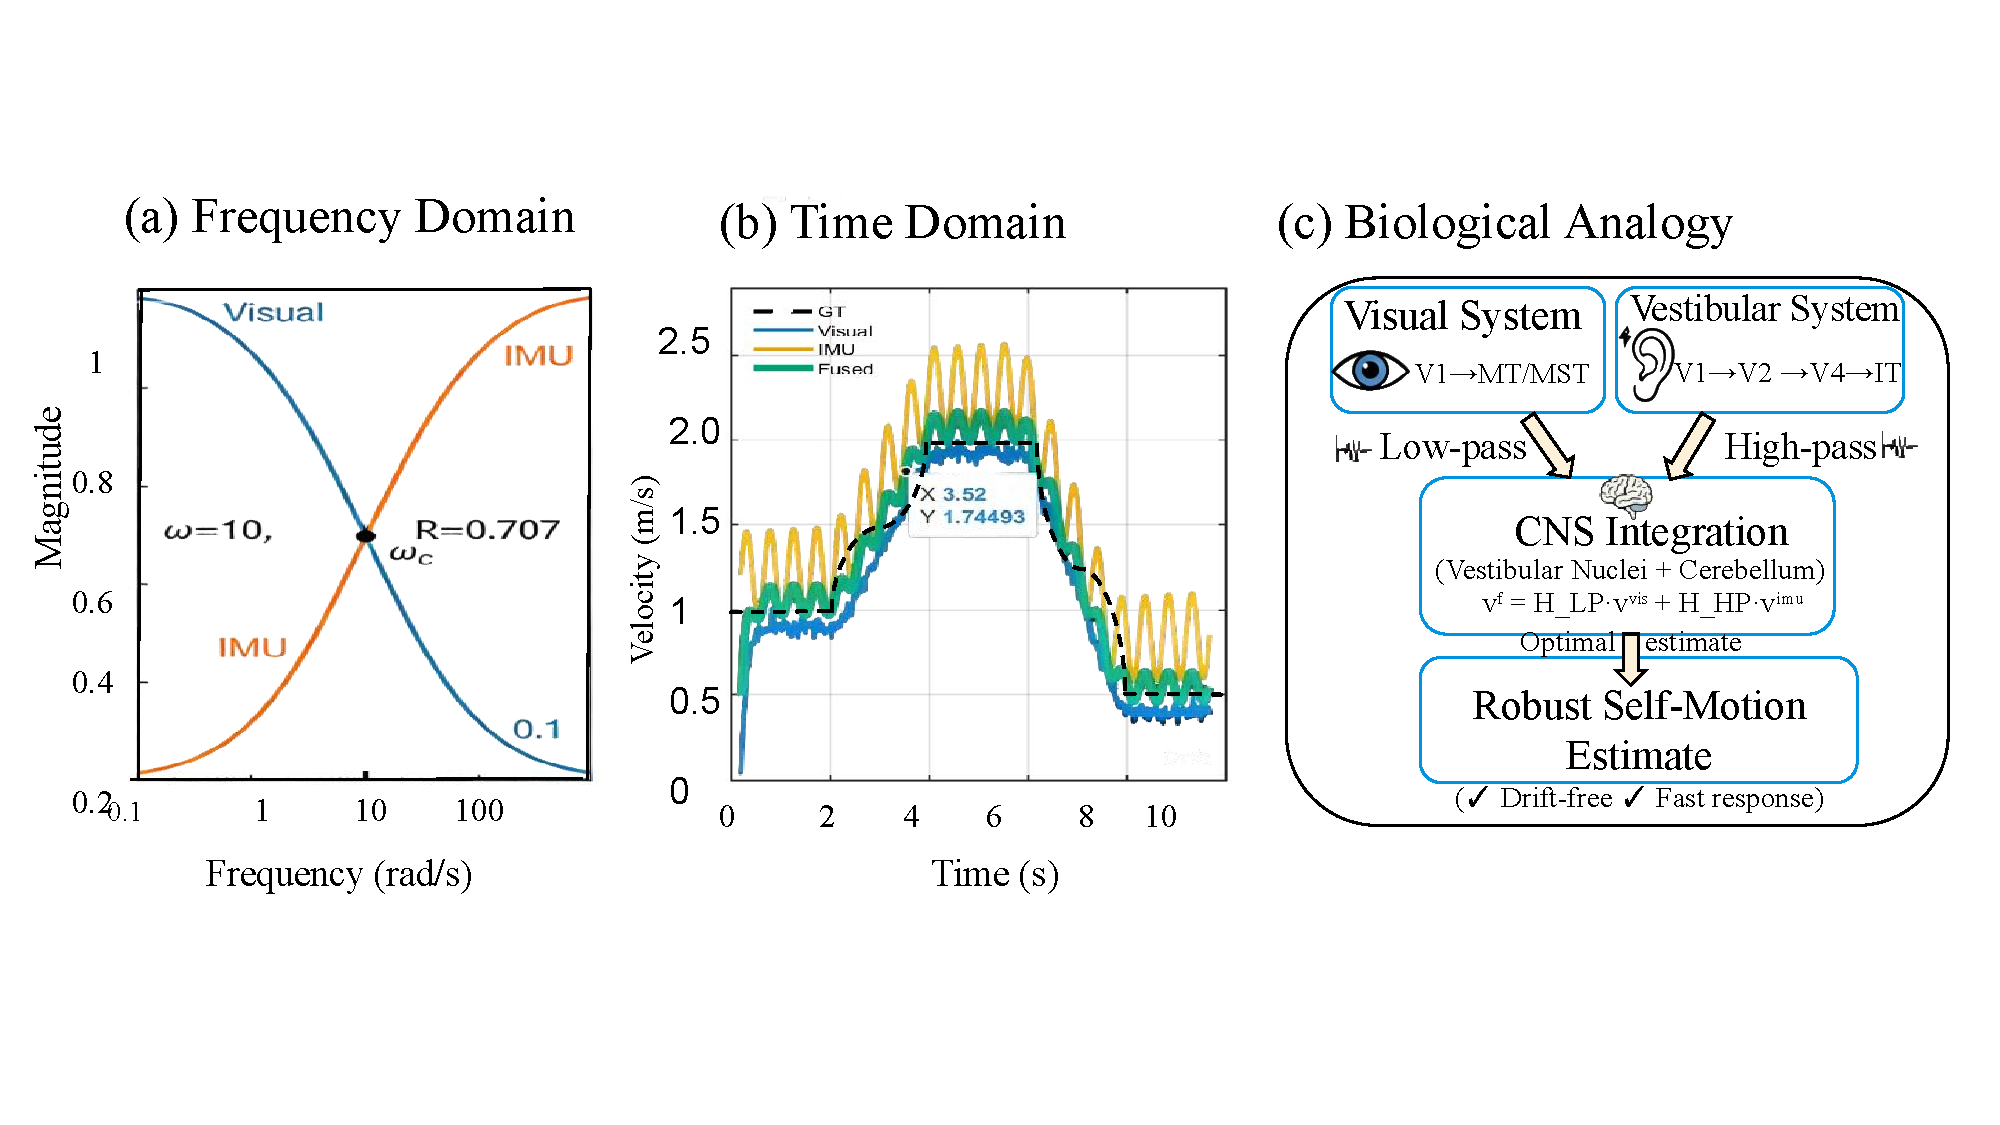
\includegraphics[width=\textwidth]{fig/imu_visual_complementary_fusion.pdf}
    \caption{Com\-ple\-men\-tary IMU-visual fusion architecture. (a) Frequency domain analysis showing complementary filter characteristics. (b) Time domain signal comparison. (c) Biological analogy to ves\-tib\-u\-lar-visual integration in the CNS.}
    \label{fig:imu_visual_fusion}
\end{figure*}

\textbf{Filter Design.} Let $\mathcal{L}_\tau$ denote a low-pass filter with time constant $\tau$, and $\mathcal{H}_\tau$ denote the complementary high-pass filter satisfying $\mathcal{L}_\tau + \mathcal{H}_\tau = \mathrm{Id}$ (identity). The fused velocity and yaw rate are:
\begin{align}
    \text{Low-pass: }  & \;L_t = \alpha L_{t-1} + (1-\alpha) x_t,\quad L_0=0 \\
    \text{High-pass: } & \;H_t = x_t - L_t
\end{align}
where $\alpha$ is IIR filter forgetting factor, $L_t$ stores low-frequency smoothed signal, and $H_t$ stores residual high-frequency signal component.
\textbf{Biological Analogy.} This fusion strategy mirrors multisensory integration in the ves\-tib\-u\-lar nuclei and posterior parietal cortex (area 7a), where visual and ves\-tib\-u\-lar signals are combined to estimate self-motion. Neurons in these regions exhibit weighted combinations of visual and ves\-tib\-u\-lar tuning, with dynamic weighting depending on signal reliability---analogous to our fixed weighting parameters $\eta$ and $\eta_r$.

\textbf{Discrete-Time Implementation.} With sampling interval $\Delta t$, we implement first-order IIR (infinite impulse response) filters. Choose forgetting factors $\alpha=\exp(-\Delta t/\tau)$ and $\alpha_r=\exp(-\Delta t/\tau_r)$. For any input sequence $x_t$, define:
\begin{align}
    \text{Low-pass: }  & \;L_t = \alpha L_{t-1} + (1-\alpha) x_t,\quad L_0=0 \\
    \text{High-pass: } & \;H_t = x_t - L_t
\end{align}
Then the fused cues are computed as:
\begin{align}
    \mathbf{v}^\mathrm{f}_t & = (1-\eta)\,L^\mathrm{vis}_t + \eta\,H^\mathrm{imu}_t \\
    r^\mathrm{f}_t          & = (1-\eta_r)\,L^{r,vis}_t + \eta_r\,H^{r}_t
\end{align}
where $L^\mathrm{vis}_t$ and $H^\mathrm{imu}_t$ denote the low-pass filtered visual velocity and high-pass filtered IMU velocity, respectively, and similarly for the yaw rates.

\textbf{Frequency-Domain Transfer Functions.} In the Laplace domain with $s = j\omega$ (frequency variable), the first-order low-pass and high-pass filters have transfer functions:
\begin{align}
    H_{LP}(s) & = \frac{1}{1 + \tau s} = \frac{1/\tau}{s + 1/\tau}, \label{eq:h_lp} \\
    H_{HP}(s) & = \frac{\tau s}{1 + \tau s} = \frac{s}{s + 1/\tau}, \label{eq:h_hp}
\end{align}
satisfying $H_{LP}(s) + H_{HP}(s) = 1$ (unity gain at all frequencies). The cutoff frequency $\omega_c = 1/\tau$ separates low- and high-frequency regions: for $\omega \ll \omega_c$, $|H_{LP}| \approx 1$ and $|H_{HP}| \approx 0$ so the visual pathway dominates (drift-free, slower dynamics); whereas for $\omega \gg \omega_c$, $|H_{LP}| \approx 0$ and $|H_{HP}| \approx 1$, so IMU cues dominate (fast but drifting).

With $\tau = 0.1$s, the cutoff frequency is $\omega_c = 10$ rad/s ($\approx 1.6$ Hz), ensuring IMU handles high-frequency motion ($>$2 Hz, e.g., vibrations, rapid turns) while vision corrects low-frequency drift ($<$1 Hz). This mimics biological ves\-tib\-u\-lar-visual integration where ves\-tib\-u\-lar organs respond to frequencies 0.1-10 Hz and visual motion perception dominates below 0.5 Hz \cite{Angelaki2004}.

\textbf{Computational Efficiency.} This implementation requires only two state variables per signal (current low-pass filter state $L_t$ and previous value $L_{t-1}$) and involves simple scalar multiplications and additions. The computational cost is $\mathcal{O}(1)$ per update, making it suitable for real-time embedded implementation---a stark contrast to the $\mathcal{O}(n^3)$ matrix inversions required by Extended Kalman Filters for tightly-coupled visual-inertial odometry.

\textbf{Adaptive Weighting.} While our baseline implementation uses fixed fusion weights $\eta$ and $\eta_r$, the framework naturally extends to adaptive weighting based on signal reliability. For instance, during aggressive maneuvers or rapid lighting changes, visual odometry may become unreliable, warranting increased reliance on IMU ($\eta \to 1$). Conversely, during slow motion where IMU integration accumulates bias, visual odometry should dominate ($\eta \to 0$). Adaptive schemes can be implemented by:
\begin{equation}
    \eta_t = f(\sigma^\mathrm{vis}_t, \sigma^\mathrm{imu}_t),\quad \text{e.g.} \quad \eta_t = \frac{\sigma^\mathrm{vis}_t}{\sigma^\mathrm{vis}_t + \sigma^\mathrm{imu}_t}
\end{equation}
where $\sigma_t^\mathrm{vis}$ and $\sigma_t^\mathrm{imu}$ are real-time uncertainty estimations of visual and inertial measurements, and $\eta_t$ is time-varying fusion weight.

Additionally, the visual odometry scale factor $\kappa_t$ in Eq.~(202) can be adapted to maintain consistency between visual and inertial velocity magnitudes:
\begin{equation}
    \kappa_{t+1} = \kappa_t \cdot \left(1 + \beta \frac{\lVert\mathbf{v}^\mathrm{imu}_t\rVert - \lVert\kappa_t \bar{\mathbf{v}}^\mathrm{vis}_t\rVert}{\lVert\kappa_t \bar{\mathbf{v}}^\mathrm{vis}_t\rVert}\right)
\end{equation}
where $\beta$ is small constant gain for online visual odometry scale correction.

with small adaptation gain $\beta \ll 1$ (e.g., $\beta=0.01$). This online scale adaptation compensates for systematic errors in the assumed ground plane depth or camera calibration inaccuracies.

\subsection{Neural Spatial Representation}

The spatial representation module encodes the robot's 4-DoF pose through bio-inspired neural coordinate systems using conjunctive pose cells. The 3D location $(x, y, z)$ is represented by grid cells using a 3D continuous attractor network (MD-CAN), while orientation $\psi$ (yaw) is encoded by multilayered head direction cells. These representations enable stable, noise-tolerant path integration through attractor dynamics.

\textbf{3D Grid Cell Network.} The 3D grid cell network mimics the 3D spatial neural representation in the mammalian brain, exhibiting regular 3D lattice patterns (face-centered cubic, FCC) that encode position and provide a universal metric for path integration. Inspired by the discovery of 3D grid cells in bats~\cite{finkelstein2016three} and theoretical models of hexagonal grid structures~\cite{hafting2005microstructure}, our implementation extends 2D continuous attractor networks to full 3D space while preserving key biological properties: multi-scale representation, metric path integration, and resilience to noise.

\textbf{Network Architecture.} The 3D grid cell network is a 3D multi-scale continuous attractor network (MD-CAN) with dimensions $N_x \times N_y \times N_z$ (typically $N_x = N_y = N_z = 61$). The network activity $\mathbf{A}^\mathrm{g}_t \in \mathbb{R}^{N_x \times N_y \times N_z}$ represents a distributed population code for the robot's 3D position $(x_t, y_t, z_t)$, where each cell $(i,j,k)$ is tuned to a preferred spatial location within the environment. The activity forms a localized ``bump'' (or activity packet) centered at the current position, analogous to the activity bump observed in rodent entorhinal cortex recordings.

The network's topology implements periodic boundary conditions with toroidal wrapping, enabling unbounded spatial representation. Cell-to-cell connectivity follows a face-centered cubic (FCC) lattice---the densest sphere packing in 3D---which provides optimal spatial coverage with minimal neurons. In the FCC structure, each cell has 12 nearest neighbors (compared to 6 in 2D hexagonal grids), yielding efficient 3D path integration with isotropic directional sensitivity.

\begin{figure*}[!t]
    \centering
    \includegraphics[width=\textwidth]{fig/3D_grid_cell_fcc_lattice.pdf}
    \caption{3D Grid Cell Network with FCC lattice structure. (a) 3D activity packet representing position $(x,y,z)$ through distributed population code. (b) FCC lattice structure showing hexagonal grid pattern with three height layers for dense 3D packing. (c) 4-DoF encoding scheme combining position and heading representations.}
    \label{fig:3D_grid_cell_fcc}
\end{figure*}

Figure~\ref{fig:3D_grid_cell_fcc} schematically illustrates: (a) the 3D activity bump at position $(x, y, z)$, represented as isosurfaces to visualize the localized excitation; (b) the FCC lattice projected onto the 2D plane, showing the characteristic hexagonal pattern arising from layer-offset positioning, where different height layers (indicated by color) are displaced by half-lattice constants to achieve optimal packing; (c) the complete 4-DoF encoding pipeline integrating position and heading representations.

\textbf{Continuous Attractor Dynamics.} The network maintains a localized ``bump'' of activity through three key mechanisms:

\textbf{(1) Local excitation.} Cells excite their neighbors according to a Gaussian connectivity kernel. With a separable kernel
\begin{equation}
    \mathcal{K}^\mathrm{g}_{a,b,c}=\mathcal{N}(a;0,\sigma_x)\mathcal{N}(b;0,\sigma_y)\mathcal{N}(c;0,\sigma_z)
\end{equation}
where $\mathcal{N}(\cdot;\mu,\sigma)$ denotes one-dimensional Gaussian distribution, and $\sigma_x,\sigma_y,\sigma_z$ are spatial kernel widths along three axes.
the excitatory update is:
\begin{equation}
    \Delta A^\mathrm{g}_{i,j,k}=\sum_{p,q,r} A^\mathrm{g}_{p,q,r}\,\mathcal{K}^\mathrm{g}_{\langle i-p\rangle_{N_x},\langle j-q\rangle_{N_y},\langle k-r\rangle_{N_z}}
\end{equation}
where $\langle \cdot \rangle_N$ denotes modulo-$N$ wrapping for periodic boundary conditions. Typical parameters are $\sigma_x = \sigma_y = \sigma_z = 5$ cells.

\textbf{(2) Global inhibition and normalization.} Uniform global inhibition subtracts the mean activity, while rectification and normalization maintain a single stable bump:
\begin{equation}
    A^\mathrm{g}_{i,j,k}\leftarrow \big[A^\mathrm{g}_{i,j,k}+\Delta A^\mathrm{g}_{i,j,k}-\lambda\,\bar A^\mathrm{g}\big]_+,\quad \bar A^\mathrm{g}=\frac{1}{N_xN_yN_z}\sum_{p,q,r}A^\mathrm{g}_{p,q,r}
\end{equation}
where $[\cdot]_+ = \max(0, \cdot)$ is rectification and $\lambda$ controls inhibition strength (typically $\lambda=1.0$). After inhibition, the activity is $L_1$-normalized:
\begin{equation}
    A^\mathrm{g}\leftarrow \frac{A^\mathrm{g}}{\lVert A^\mathrm{g}\rVert_1}=\frac{A^\mathrm{g}}{\sum_{i,j,k}|A^\mathrm{g}_{i,j,k}|}
\end{equation}
This normalization ensures the activity pattern has unit total mass, making the readout (center of mass) insensitive to overall activity magnitude.

\textbf{(3) Path integration.} The activity bump shifts according to fused velocity cues $\mathbf{v}^\mathrm{f}_t = (v^f_x, v^f_y, v^f_z)$. Index shifts are computed as:
\begin{equation}
    (\Delta i,\Delta j,\Delta k)=\big(\lfloor \gamma_x v^f_x\Delta t\rfloor,\ \lfloor \gamma_y v^f_y\Delta t\rfloor,\ \lfloor \gamma_z v^f_z\Delta t\rfloor\big)
\end{equation}
where $\gamma_x,\gamma_y,\gamma_z$ are metric-to-index gain factors converting physical velocity to network grid shifts.
\begin{equation}
    A^\mathrm{g}_{i,j,k}\leftarrow A^\mathrm{g}_{\langle i-\Delta i\rangle_{N_x},\langle j-\Delta j\rangle_{N_y},\langle k-\Delta k\rangle_{N_z}}
\end{equation}
This discrete shifting operation efficiently implements path integration on the toroidal network topology.

\textbf{Visual Anchoring and Drift Correction.} Pure path integration accumulates drift over time. To prevent unbounded error, the grid cell activity is anchored to visual landmarks through learned associations. Let $\Xi_{m,i,j,k}$ store the association strength between visual template $m$ and grid cell $(i,j,k)$. For each active visual template $m \in \mathcal{S}_{active}$, update associations and inject corrective activity:
\begin{align}
     & \text{Hebbian learning: } \Xi_{m,i,j,k}^{t+1}=\max\big(\eta\,VT_m\,A^\mathrm{g}_{i,j,k},\ \Xi_{m,i,j,k}^{t}\big)                                             \\
     & \text{Corrective injection: } \Delta A^\mathrm{g}_{i,j,k} \mathrel{+}= \frac{\rho}{|\mathcal{S}_{active}|}\sum_{m\in\mathcal{S}_{active}}VT_m\,\Xi_{m,i,j,k}
\end{align}
where $\eta$ is Hebbian learning rate, $\rho$ is spatial correction strength, and $\mathcal{S}_{active}$ is set of currently matched visual templates.

\textbf{Multilayered Head Direction Cells.} The multilayered head direction cell (HDC) network represents the robot's orientation using a 2D MD-CAN with dimensions $N_\psi \times N_h$ (azimuth bins by height layers). Different height layers allow representation of heading at various vertical positions, supporting 3D operation where orientation may vary with altitude.

\textbf{Network Architecture.} The multilayer head-direction network has activity $\mathbf{A}^\mathrm{h} \in \mathbb{R}^{N_\psi \times N_h}$ (typically $N_\psi = 360$ azimuth bins and $N_h = 5$ height layers). Each cell $(u, h)$ is tuned to azimuth angle $\theta_u = 2\pi u / N_\psi$ and height layer $h$.

\textbf{Attractor Dynamics.} Similar to the grid cell network, the HDC network employs local excitation, global inhibition, and path integration. With a Gaussian kernel $\mathcal{K}^\mathrm{h}$:
\begin{equation}
    \Delta A^\mathrm{h}_{\psi,h}=\sum_{u,v}A^\mathrm{h}_{u,v}\,\mathcal{K}^\mathrm{h}_{\langle \psi-u\rangle_{N_\psi},\langle h-v\rangle_{N_h}}
\end{equation}
followed by inhibition and normalization:
\begin{equation}
    A^\mathrm{h}\leftarrow \frac{[A^\mathrm{h}+\Delta A^\mathrm{h}-\lambda_h\,\bar A^\mathrm{h}]_+}{\lVert A^\mathrm{h}\rVert_1}
\end{equation}
Path integration shifts the activity bump according to yaw rate $r^f$ and vertical velocity $v^f_z$:
\begin{equation}
    \Delta\psi=\lfloor \gamma_\psi r^f \Delta t\rfloor,\quad \Delta h=\lfloor \gamma_h v^f_z \Delta t\rfloor
\end{equation}
where $\gamma_\psi$ converts angular velocity to azimuth bins, and $\gamma_h$ maps vertical velocity to height layer shifts.
\textbf{Pose Readout.} The metric pose estimate is decoded from the spatial cell activities via center-of-mass computation (population vector decoding):
\begin{align}
    \hat{\mathbf{p}}_t & = ({\hat x}_t, {\hat y}_t, {\hat z}_t) = \frac{\sum_{i,j,k} \mathbf{c}_{i,j,k} A^\mathrm{g}_{i,j,k,t}}{\sum_{i,j,k} A^\mathrm{g}_{i,j,k,t}}, \quad \mathbf{c}_{i,j,k} = (x_i, y_j, z_k) \\
    \hat{\psi}_t       & = \mathrm{\mathrm{atan2}}\left(\sum_{u,h} A^\mathrm{h}_{u,h,t} \sin\theta_u, \sum_{u,h} A^\mathrm{h}_{u,h,t} \cos\theta_u\right), \quad \theta_u = 2\pi u / N_\psi
\end{align}
This decoding naturally handles the circular topology of orientation (using $\mathrm{\mathrm{atan2}}$ to avoid angle wrapping issues) and provides sub-bin resolution for position through the weighted average.

\subsection{Experience Map and Loop Closure}

The multilayered experience map represents 3D spatial experiences as a graph structure, providing a hybrid topological-metric representation that combines the benefits of discrete place-based maps (topological robustness, loop closure) and continuous metric representations (accurate localization).

\textbf{Experience Representation.} Each experience node $\mathcal{E}_i$ encodes a distinct spatial episode comprising the active visual template and descriptor $(VT_i,\,\boldsymbol{\phi}_i\in\mathbb{R}^{4096})$, the concurrent spatial-cell codes $\mathbf{P}^{gc}_i=\mathbf{A}^\mathrm{g}_i\in\mathbb{R}^{N_x\times N_y\times N_z}$ and $\mathbf{P}^{hdc}_i=\mathbf{A}^\mathrm{h}_i\in\mathbb{R}^{N_\psi\times N_h}$, the metric pose $(x_i, y_i, z_i, \psi_i)$ decoded from these activities, and the timestamp $t_i$ for temporal ordering.
This rich multimodal encoding enables robust loop closure detection through visual matching while maintaining metric information through the spatial cell codes.

\textbf{Experience Creation and Linking.} As the robot navigates, new experiences are created when the current spatial representation differs sufficiently from all existing experiences. The creation criterion combines visual and spatial cell similarity:
\begin{equation}
    \begin{aligned}
        \text{Create new experience if }\; & d_{cos}(\boldsymbol{\phi}_t, \boldsymbol{\phi}_j) > \tau_{VT} \quad \text{for all } j \in \mathcal{E} \\
                                           & \text{or } \lVert (\hat{x}_t, \hat{y}_t, \hat{z}_t) - (x_j, y_j, z_j) \rVert > d_{thresh}
    \end{aligned}
\end{equation}
where $\tau_{VT} = 0.08$ is the visual template matching threshold and $d_{thresh}$ is a spatial distance threshold (typically 0.5~m).

Consecutive experiences are linked by directed edges encoding the relative pose transition:
\begin{equation}
    \mathbf{T}_{i \to i+1} = (\Delta x, \Delta y, \Delta z, \Delta \psi) = (x_{i+1} - x_i, y_{i+1} - y_i, z_{i+1} - z_i, \psi_{i+1} - \psi_i)
\end{equation}
These edges form the primary topological structure of the experience map graph $\mathcal{G} = (\mathcal{V}, \mathcal{E})$.

\textbf{Loop Closure Detection.} Loop closure is detected when the current visual template matches a previous experience beyond a minimum temporal separation (to avoid trivial closures):
\begin{equation}
    \begin{aligned}
        \text{Loop closure detected if } \exists j:\; & d_{cos}(\boldsymbol{\phi}_t, \boldsymbol{\phi}_j) < \tau_{loop} \\
                                                      & |t - t_j| > T_{min}
    \end{aligned}
\end{equation}
where $\tau_{loop} = 0.05$ (stricter than the template creation threshold to reduce false positives) and $T_{min} = 50$ frames (approximately 5 seconds at 10 Hz).

Upon detecting a loop closure, a loop edge is added to the graph with the pose residual:
\begin{equation}
    \mathbf{T}_{loop} = (\hat{x}_t - x_j, \hat{y}_t - y_j, \hat{z}_t - z_j, \hat{\psi}_t - \psi_j)
\end{equation}
This loop constraint typically violates graph consistency (due to accumulated drift), triggering map relaxation.

\textbf{Map Relaxation.} Map relaxation distributes the loop closure error across all experiences along the loop path to minimize global inconsistency. We employ an iterative relaxation algorithm:

\textbf{Step 1: Identify loop path.} Given a loop closure edge from experience $j$ to experience $t$, identify the sequence of experiences $\mathcal{P} = \{j, j+1, \ldots, t-1, t\}$ along the path.

\textbf{Step 2: Compute pose residual.} The accumulated pose transition along the loop should ideally close (return to the origin):
\begin{equation}
    \mathbf{e}_{loop} = \sum_{k \in \mathcal{P}} \mathbf{T}_{k \to k+1} - \mathbf{T}_{loop}
\end{equation}
where $\mathbf{e}_{loop}$ is accumulated pose drift residual around closed trajectory, and $\mathcal{P}$ denotes ordered experience sequence forming the loop.
\textbf{Step 3: Distribute correction.} Distribute the correction proportionally across the loop experiences:
\begin{equation}
    \mathbf{T}_{k \to k+1} \leftarrow \mathbf{T}_{k \to k+1} - \frac{\mathbf{e}_{loop}}{|\mathcal{P}|}
\end{equation}
This uniform distribution assumes drift accumulates at a constant rate, a reasonable first-order approximation.

\textbf{Step 4: Update experience poses.} Recompute all experience poses by integrating the corrected transitions:
\begin{equation}
    (x_{k+1}, y_{k+1}, z_{k+1}, \psi_{k+1}) = (x_k, y_k, z_k, \psi_k) + \mathbf{T}_{k \to k+1}
\end{equation}

\textbf{Step 5: Re-anchor spatial cells.} Inject the corrected pose $(\hat{x}, \hat{y}, \hat{z}, \hat{\psi})_{corr}$ back into the spatial cell networks by reinitializing the activity bumps at the corrected locations. This ``resets'' the path integration from the corrected reference, preventing error accumulation in subsequent operation.

This relaxation procedure runs iteratively until convergence or a maximum number of iterations, ensuring the experience map remains globally consistent while preserving local metric accuracy.

